\documentclass{standalone}
\usepackage{tikz}
\usetikzlibrary{patterns, positioning}


\begin{document}
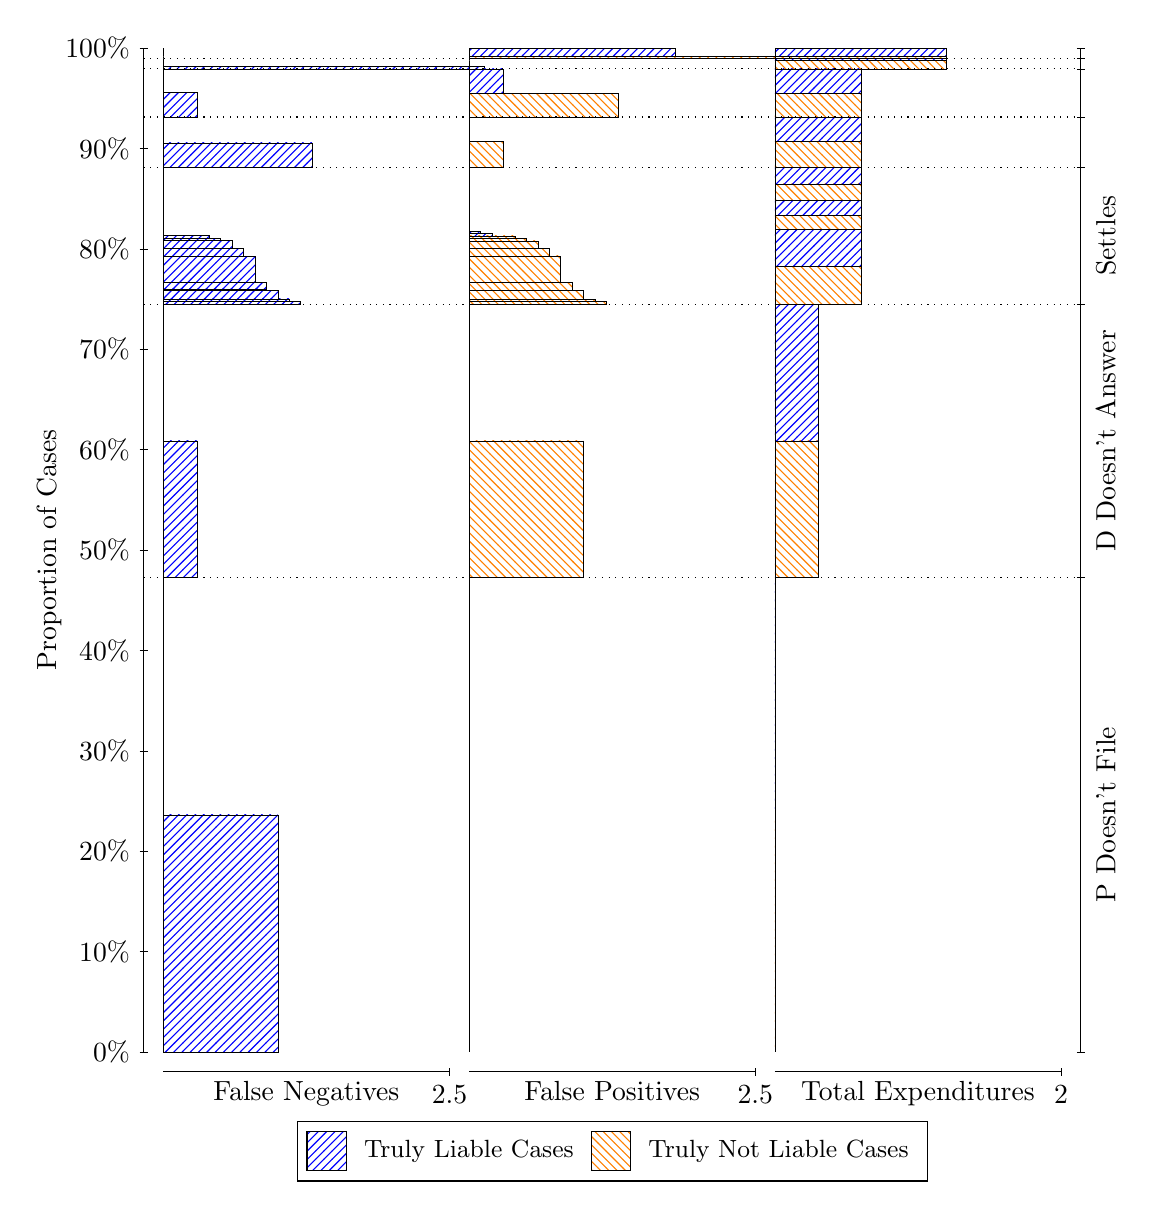
\begin{tikzpicture}
\draw[black, very thin] (1.5,1.75) -- (1.5,14.5);
\node[rotate=90, text=black, anchor=center] at (0.3, 8.125) {Proportion of Cases};
\draw[black, very thin] (1.45,1.75) -- (1.55,1.75);
\node[text=black, anchor=east] at (1.45, 1.75) {0\%};
\draw[black, very thin] (1.45,3.025) -- (1.55,3.025);
\node[text=black, anchor=east] at (1.45, 3.025) {10\%};
\draw[black, very thin] (1.45,4.3) -- (1.55,4.3);
\node[text=black, anchor=east] at (1.45, 4.3) {20\%};
\draw[black, very thin] (1.45,5.575) -- (1.55,5.575);
\node[text=black, anchor=east] at (1.45, 5.575) {30\%};
\draw[black, very thin] (1.45,6.85) -- (1.55,6.85);
\node[text=black, anchor=east] at (1.45, 6.85) {40\%};
\draw[black, very thin] (1.45,8.125) -- (1.55,8.125);
\node[text=black, anchor=east] at (1.45, 8.125) {50\%};
\draw[black, very thin] (1.45,9.4) -- (1.55,9.4);
\node[text=black, anchor=east] at (1.45, 9.4) {60\%};
\draw[black, very thin] (1.45,10.675) -- (1.55,10.675);
\node[text=black, anchor=east] at (1.45, 10.675) {70\%};
\draw[black, very thin] (1.45,11.95) -- (1.55,11.95);
\node[text=black, anchor=east] at (1.45, 11.95) {80\%};
\draw[black, very thin] (1.45,13.225) -- (1.55,13.225);
\node[text=black, anchor=east] at (1.45, 13.225) {90\%};
\draw[black, very thin] (1.45,14.5) -- (1.55,14.5);
\node[text=black, anchor=east] at (1.45, 14.5) {100\%};

\draw[black, very thin] (13.4,1.75) -- (13.4,14.5);
\draw[black, very thin] (13.35,1.75) -- (13.45,1.75);
\node[anchor=west] at (13.35, 1.75) {};
\draw[black, very thin] (13.35,7.7724) -- (13.45,7.7724);
\node[anchor=west] at (13.35, 7.7724) {};
\draw[black, very thin] (13.35,11.248) -- (13.45,11.248);
\node[anchor=west] at (13.35, 11.248) {};
\draw[black, very thin] (13.35,12.985) -- (13.45,12.985);
\node[anchor=west] at (13.35, 12.985) {};
\draw[black, very thin] (13.35,13.624) -- (13.45,13.624);
\node[anchor=west] at (13.35, 13.624) {};
\draw[black, very thin] (13.35,14.235) -- (13.45,14.235);
\node[anchor=west] at (13.35, 14.235) {};
\draw[black, very thin] (13.35,14.368) -- (13.45,14.368);
\node[anchor=west] at (13.35, 14.368) {};
\draw[black, very thin] (13.35,14.5) -- (13.45,14.5);
\node[anchor=west] at (13.35, 14.5) {};

\draw[black, very thin, pattern color=blue, pattern=north east lines] (1.75,1.75) rectangle (3.2033,4.7612);
\draw[black, very thin, pattern color=orange, pattern=north west lines] (1.75,4.7612) rectangle (1.75,7.7724);
\draw[black, very thin, pattern color=blue, pattern=north east lines] (1.75,7.7724) rectangle (2.186,9.51);
\draw[black, very thin, pattern color=orange, pattern=north west lines] (1.75,9.51) rectangle (1.75,11.248);
\draw[black, very thin, pattern color=blue, pattern=north east lines] (1.75,11.248) rectangle (3.494,11.283);
\draw[black, very thin, pattern color=blue, pattern=north east lines] (1.75,11.283) rectangle (3.3487,11.313);
\draw[black, very thin, pattern color=blue, pattern=north east lines] (1.75,11.313) rectangle (3.2033,11.422);
\draw[black, very thin, pattern color=blue, pattern=north east lines] (1.75,11.422) rectangle (3.058,11.442);
\draw[black, very thin, pattern color=blue, pattern=north east lines] (1.75,11.442) rectangle (3.058,11.521);
\draw[black, very thin, pattern color=blue, pattern=north east lines] (1.75,11.521) rectangle (2.9127,11.857);
\draw[black, very thin, pattern color=blue, pattern=north east lines] (1.75,11.857) rectangle (2.7673,11.954);
\draw[black, very thin, pattern color=blue, pattern=north east lines] (1.75,11.954) rectangle (2.622,12.059);
\draw[black, very thin, pattern color=blue, pattern=north east lines] (1.75,12.059) rectangle (2.4767,12.087);
\draw[black, very thin, pattern color=blue, pattern=north east lines] (1.75,12.087) rectangle (2.3313,12.119);
\draw[black, very thin, pattern color=orange, pattern=north west lines] (1.75,12.119) rectangle (1.75,12.985);
\draw[black, very thin, pattern color=blue, pattern=north east lines] (1.75,12.985) rectangle (3.6393,13.294);
\draw[black, very thin, pattern color=orange, pattern=north west lines] (1.75,13.294) rectangle (1.75,13.624);
\draw[black, very thin, pattern color=blue, pattern=north east lines] (1.75,13.624) rectangle (2.186,13.937);
\draw[black, very thin, pattern color=orange, pattern=north west lines] (1.75,13.937) rectangle (1.75,14.235);
\draw[black, very thin, pattern color=blue, pattern=north east lines] (1.75,14.235) rectangle (5.8193,14.262);
\draw[black, very thin, pattern color=orange, pattern=north west lines] (1.75,14.262) rectangle (1.75,14.368);
\draw[black, very thin, pattern color=orange, pattern=north west lines] (1.75,14.368) rectangle (1.75,14.395);
\draw[black, very thin, pattern color=blue, pattern=north east lines] (1.75,14.395) rectangle (1.75,14.5);
\draw[black, very thin, pattern color=orange, pattern=north west lines] (5.6333,1.75) rectangle (5.6333,4.7612);
\draw[black, very thin, pattern color=blue, pattern=north east lines] (5.6333,4.7612) rectangle (5.6333,7.7724);
\draw[black, very thin, pattern color=orange, pattern=north west lines] (5.6333,7.7724) rectangle (7.0867,9.51);
\draw[black, very thin, pattern color=blue, pattern=north east lines] (5.6333,9.51) rectangle (5.6333,11.248);
\draw[black, very thin, pattern color=orange, pattern=north west lines] (5.6333,11.248) rectangle (7.3773,11.281);
\draw[black, very thin, pattern color=orange, pattern=north west lines] (5.6333,11.281) rectangle (7.232,11.311);
\draw[black, very thin, pattern color=orange, pattern=north west lines] (5.6333,11.311) rectangle (7.0867,11.423);
\draw[black, very thin, pattern color=orange, pattern=north west lines] (5.6333,11.423) rectangle (6.9413,11.526);
\draw[black, very thin, pattern color=orange, pattern=north west lines] (5.6333,11.526) rectangle (6.796,11.86);
\draw[black, very thin, pattern color=orange, pattern=north west lines] (5.6333,11.86) rectangle (6.6507,11.951);
\draw[black, very thin, pattern color=orange, pattern=north west lines] (5.6333,11.951) rectangle (6.5053,12.051);
\draw[black, very thin, pattern color=orange, pattern=north west lines] (5.6333,12.051) rectangle (6.36,12.079);
\draw[black, very thin, pattern color=orange, pattern=north west lines] (5.6333,12.079) rectangle (6.2147,12.113);
\draw[black, very thin, pattern color=blue, pattern=north east lines] (5.6333,12.113) rectangle (5.924,12.146);
\draw[black, very thin, pattern color=blue, pattern=north east lines] (5.6333,12.146) rectangle (5.7787,12.174);
\draw[black, very thin, pattern color=blue, pattern=north east lines] (5.6333,12.174) rectangle (5.6333,12.985);
\draw[black, very thin, pattern color=orange, pattern=north west lines] (5.6333,12.985) rectangle (6.0693,13.314);
\draw[black, very thin, pattern color=blue, pattern=north east lines] (5.6333,13.314) rectangle (5.6333,13.624);
\draw[black, very thin, pattern color=orange, pattern=north west lines] (5.6333,13.624) rectangle (7.5227,13.921);
\draw[black, very thin, pattern color=blue, pattern=north east lines] (5.6333,13.921) rectangle (6.0693,14.235);
\draw[black, very thin, pattern color=orange, pattern=north west lines] (5.6333,14.235) rectangle (5.6333,14.341);
\draw[black, very thin, pattern color=blue, pattern=north east lines] (5.6333,14.341) rectangle (5.6333,14.368);
\draw[black, very thin, pattern color=orange, pattern=north west lines] (5.6333,14.368) rectangle (9.7027,14.395);
\draw[black, very thin, pattern color=blue, pattern=north east lines] (5.6333,14.395) rectangle (8.2493,14.5);
\draw[black, very thin, pattern color=orange, pattern=north west lines] (9.5167,1.75) rectangle (9.5167,4.7612);
\draw[black, very thin, pattern color=blue, pattern=north east lines] (9.5167,4.7612) rectangle (9.5167,7.7724);
\draw[black, very thin, pattern color=orange, pattern=north west lines] (9.5167,7.7724) rectangle (10.062,9.51);
\draw[black, very thin, pattern color=blue, pattern=north east lines] (9.5167,9.51) rectangle (10.062,11.248);
\draw[black, very thin, pattern color=orange, pattern=north west lines] (9.5167,11.248) rectangle (10.607,11.724);
\draw[black, very thin, pattern color=blue, pattern=north east lines] (9.5167,11.724) rectangle (10.607,12.192);
\draw[black, very thin, pattern color=orange, pattern=north west lines] (9.5167,12.192) rectangle (10.607,12.374);
\draw[black, very thin, pattern color=blue, pattern=north east lines] (9.5167,12.374) rectangle (10.607,12.568);
\draw[black, very thin, pattern color=orange, pattern=north west lines] (9.5167,12.568) rectangle (10.607,12.776);
\draw[black, very thin, pattern color=blue, pattern=north east lines] (9.5167,12.776) rectangle (10.607,12.985);
\draw[black, very thin, pattern color=orange, pattern=north west lines] (9.5167,12.985) rectangle (10.607,13.314);
\draw[black, very thin, pattern color=blue, pattern=north east lines] (9.5167,13.314) rectangle (10.607,13.624);
\draw[black, very thin, pattern color=orange, pattern=north west lines] (9.5167,13.624) rectangle (10.607,13.921);
\draw[black, very thin, pattern color=blue, pattern=north east lines] (9.5167,13.921) rectangle (10.607,14.235);
\draw[black, very thin, pattern color=orange, pattern=north west lines] (9.5167,14.235) rectangle (11.697,14.341);
\draw[black, very thin, pattern color=blue, pattern=north east lines] (9.5167,14.341) rectangle (11.697,14.368);
\draw[black, very thin, pattern color=orange, pattern=north west lines] (9.5167,14.368) rectangle (11.697,14.395);
\draw[black, very thin, pattern color=blue, pattern=north east lines] (9.5167,14.395) rectangle (11.697,14.5);
\draw[black, dotted] (1.5,7.7724) -- (13.4,7.7724);
\draw[black, dotted] (1.5,11.248) -- (13.4,11.248);
\draw[black, dotted] (1.5,12.985) -- (13.4,12.985);
\draw[black, dotted] (1.5,13.624) -- (13.4,13.624);
\draw[black, dotted] (1.5,14.235) -- (13.4,14.235);
\draw[black, dotted] (1.5,14.368) -- (13.4,14.368);
\draw[black, very thin] (1.75,1.5) -- (5.3833,1.5);
\node[text=black, anchor=north] at (3.5667, 1.5) {False Negatives};
\draw[black, very thin] (5.3833,1.45) -- (5.3833,1.55);
\node[text=black, anchor=north] at (5.3833, 1.45) {2.5};

\draw[black, very thin] (5.6333,1.5) -- (9.2667,1.5);
\node[text=black, anchor=north] at (7.45, 1.5) {False Positives};
\draw[black, very thin] (9.2667,1.45) -- (9.2667,1.55);
\node[text=black, anchor=north] at (9.2667, 1.45) {2.5};

\draw[black, very thin] (9.5167,1.5) -- (13.15,1.5);
\node[text=black, anchor=north] at (11.333, 1.5) {Total Expenditures};
\draw[black, very thin] (13.15,1.45) -- (13.15,1.55);
\node[text=black, anchor=north] at (13.15, 1.45) {2};

\node[text=black, centered, rotate=90] at (13.72, 4.7612) {P Doesn't File};
\node[text=black, centered, rotate=90] at (13.72, 9.51) {D Doesn't Answer};
\node[text=black, centered, rotate=90] at (13.72, 12.116) {Settles};





\draw (7.449999999999999,1.5) node[draw=none] (baseCoordinate) {};
\begin{scope}[align=center]
        \matrix[scale=0.5, draw=black, below=0.5cm of baseCoordinate, nodes={draw}, column sep=0.1cm]{
            \node[rectangle, draw, minimum width=0.5cm, minimum height=0.5cm, pattern color=blue, pattern=north east lines] {}; &
            \node[draw=none, font=\small, text=black] (B) {Truly Liable Cases}; &
            \node[rectangle, draw, minimum width=0.5cm, minimum height=0.5cm, pattern color=orange, pattern=north west lines] {}; &
            \node[draw=none, font=\small, text=black] (B) {Truly Not Liable Cases}; \\
            };
\end{scope}

\end{tikzpicture}
\end{document}